\documentclass[aspectratio=169]{beamer}

\usepackage[english]{babel}
\usepackage[utf8]{inputenc}
\usepackage[T1]{fontenc}
\usepackage{lmodern}

\newcommand{\Author}{Sebastian Einsiedler}
\newcommand{\Title}{Programming for Biologist}
\newcommand{\SubTitle}{Theory and perspective}

\title{\Title}
\subtitle{\SubTitle}
\author{\Author}

\usepackage{amsmath, amssymb}
\usepackage{enumerate}
\usepackage[table]{xcolor}
\usepackage[singlespacing]{setspace}
\usepackage{hyperref}
\hypersetup{
	bookmarks=true,
	unicode=true,
	pdfauthor = {\Author},
	pdftitle = {\Title},
	pdfsubject = {\Title},
	pdfsubject = {\Author, \Title, \SubTitle Python, Programming, Programming for biologists, presentation},
	colorlinks = true,
	linkcolor = {blue!50!black},
	filecolor = {red!50!black},
	urlcolor = {blue!75!black}
}
\usepackage{csquotes}

\usepackage{footnotebackref}
\usepackage{longtable}
\usepackage{booktabs}
\usepackage{graphicx}
\usepackage{tikz}
\usepackage{listings}

\setbeamertemplate{navigation symbols}{}
\setbeamertemplate{footline}{
	\hspace{2ex}
	\insertshorttitle
	: \hspace{3em}
	\insertsectionhead
	\hfill
	\insertframenumber /
	\inserttotalframenumber
	\hspace{2ex}
	\vspace{2ex}
}
\setcounter{tocdepth}{1}
\hypersetup{bookmarksdepth = 3}

\begin{document}

\usebackgroundtemplate{
\includegraphics[width=\paperwidth]{img/Title.png}}
\begingroup
\setbeamertemplate{footline}{}
\begin{frame}{\phantom{Title}}
{
	\vskip 6em
	\color{white}
	\LARGE \Title{}
	\newline
	\large
	\SubTitle{}
	
	\vskip 5em
	\small
	\Author{}
	and 
	\color{white}{Eduard Maier} \\
	RG Neurobiology of maternal care \\
	Department Neuropeptide research in psychiatry
}
\end{frame}
\endgroup

\usebackgroundtemplate{
\includegraphics[width=\paperwidth]{img/Body.png}}

\section{Table of contents}
\begin{frame}
	\frametitle{Table of contents}
	\tableofcontents
\end{frame}

\section{Introduction}
\begin{frame}{Introduction}
Why learn how to program:
\begin{itemize}
	\item Control complex machinery
	\item Analyze large data sets
	\item Test theories by simulation
\end{itemize}
\end{frame}

\section{Course plan}
\begin{frame}{Course plan}
\begin{tabular}{ccc}
	\toprule
	Module & Content & Goal \\
	\midrule
	1 & Theory and perspective & You have an idea how programmers think \\
	2 & Fundamental building blocks & You can add numbers \\
	3 & Control structures & You can write short simple programs \\
	4 & Classes and modules & You can write more complex programs \\
	5 & Analysis and Statistics & You can apply numerical analysis to new data \\
\end{tabular}
\end{frame}

\section{Real data}
\begin{frame}{Real data}{Experiment}
\begin{figure}[h]
\centering
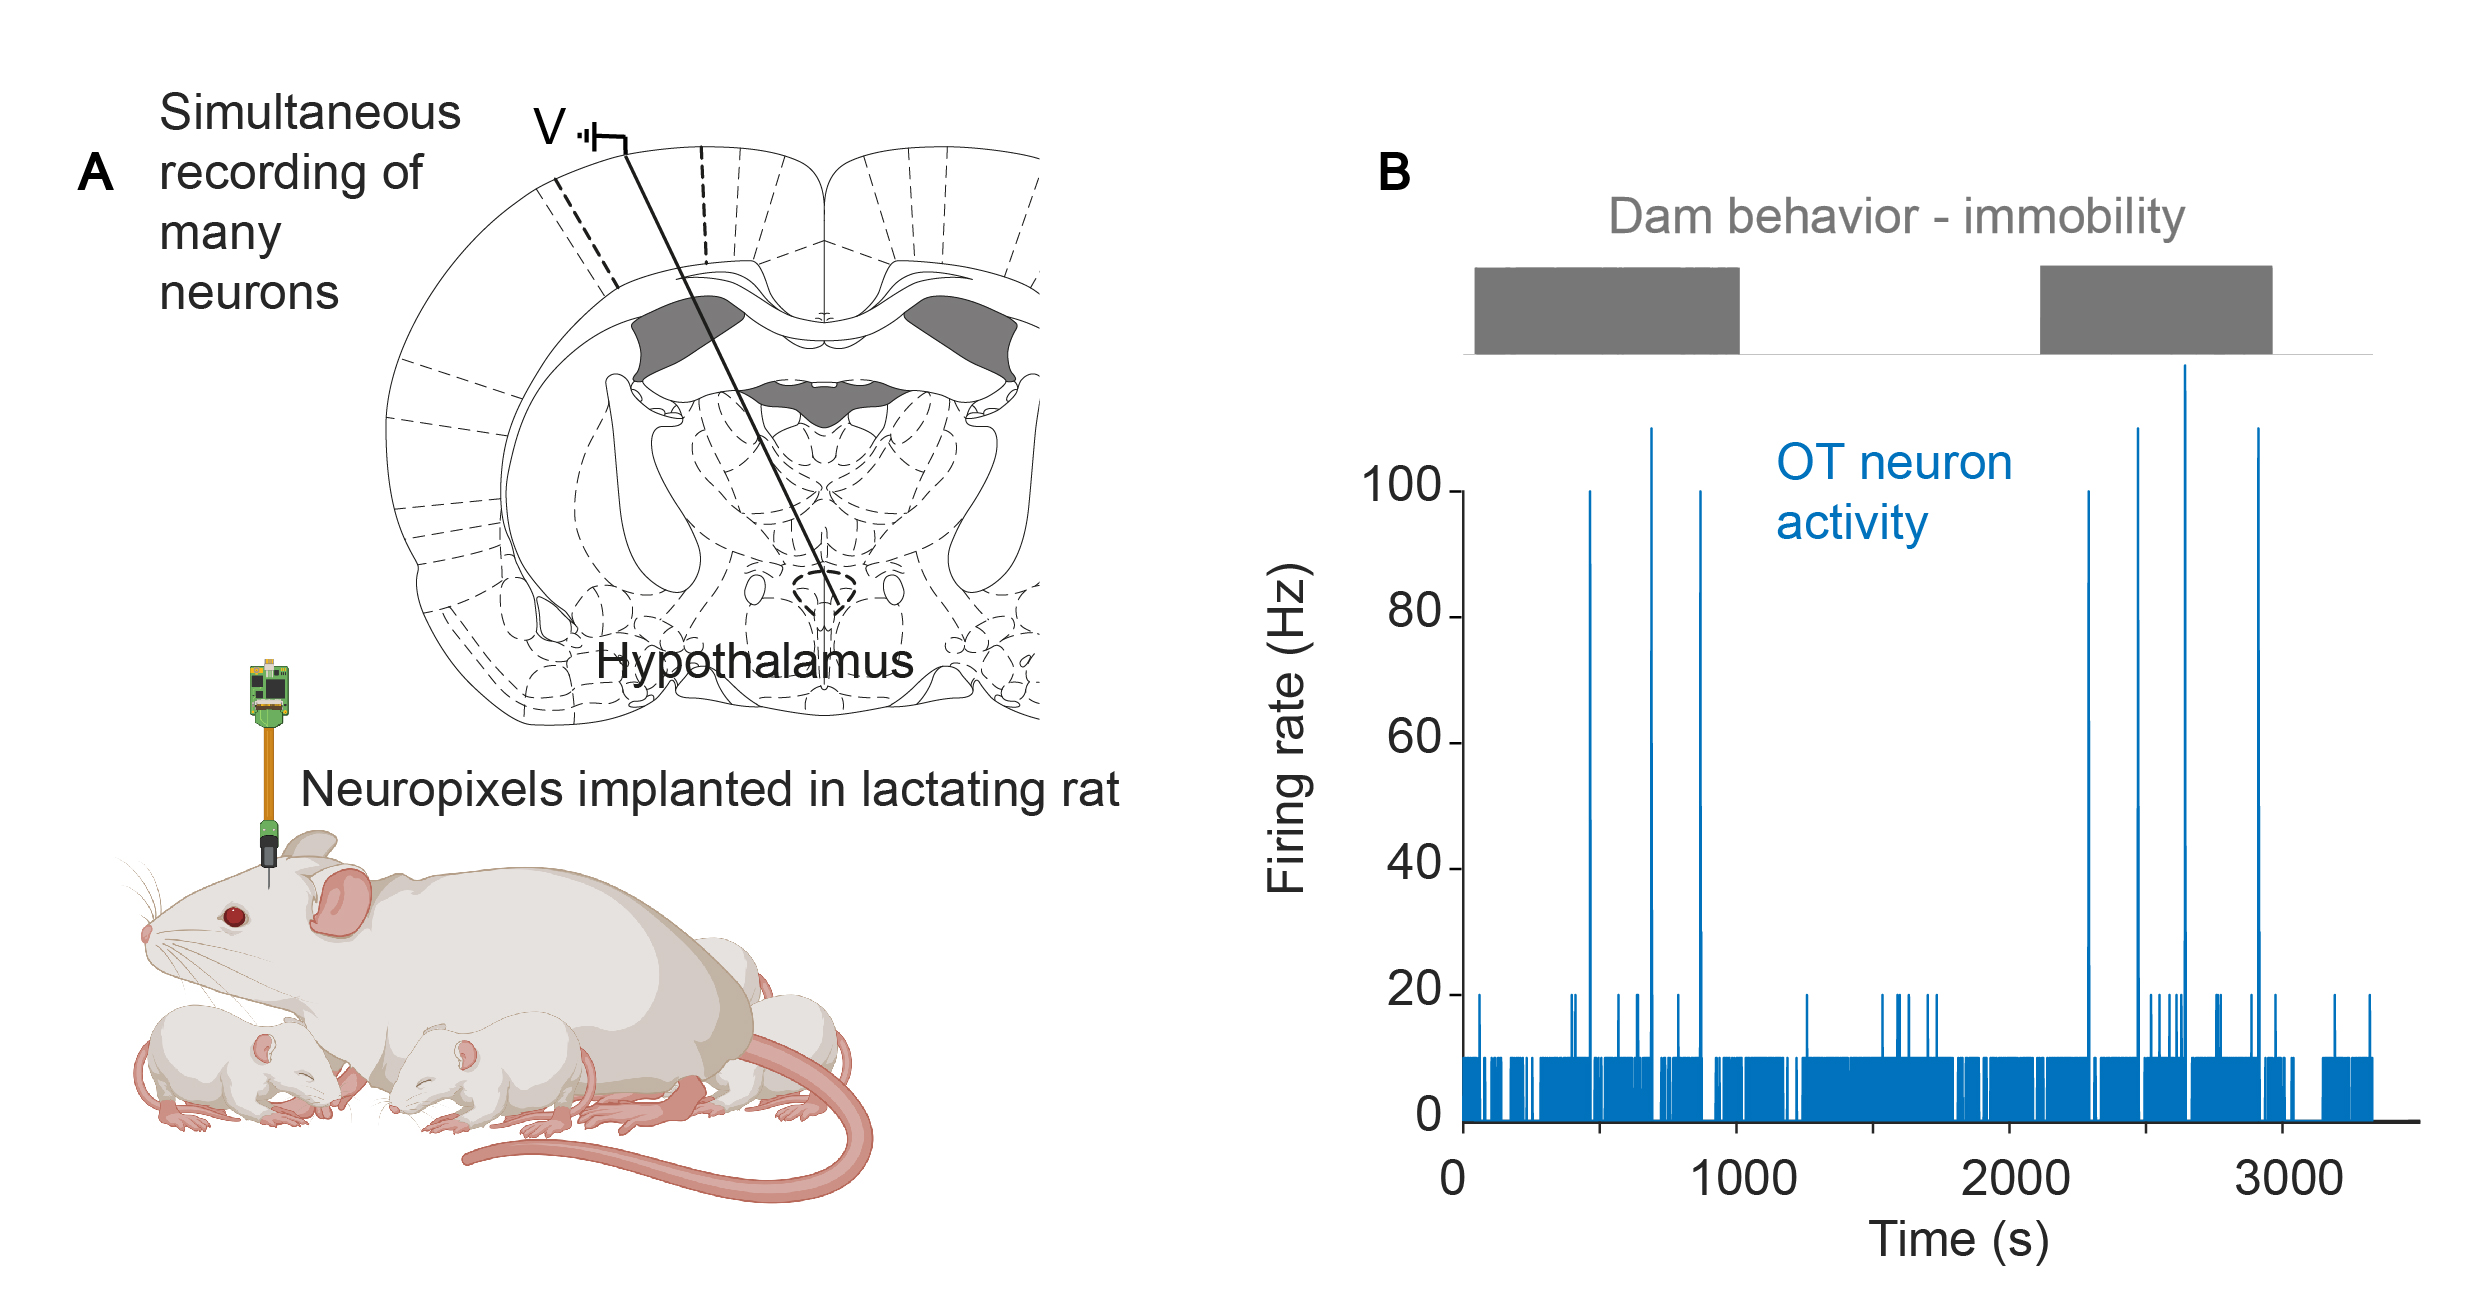
\includegraphics[width=0.5\textwidth]{../img/experiment.jpg}
\caption{
	A. Recording setup with an electrode that has many contacts along one single shank.
	B. Top: Maternal behavior (immobility vs. mobility).
	Bottom: Neural activity. Note that we see the spikes per second (Hz). 
	We also see that there are seven distinct bursts measuring around 100 spikes per second.
	Also, note that the burst pattern seen here has been described to coincide with immobility.
	The combined investigation of both neural activity and behavior thus provides converging evidence
	that the recorded neuron is an oxytocin neuron.
}
\end{figure}
\end{frame}

\begin{frame}{Real data}{Oxytocin bursts}
\begin{figure}[h]
\centering
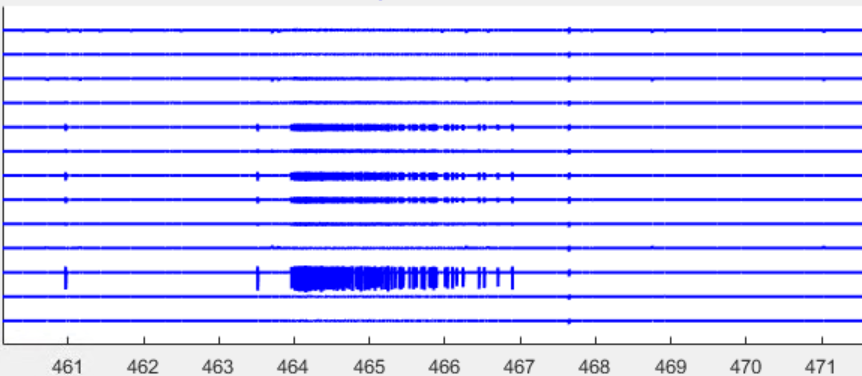
\includegraphics[width=0.8\textwidth]{../img/OTburst.png}
\caption{
	An example of an oxytocin burst consisting of multiple spikes.
	You can see a large number of spikes in the center of the image.
}
\end{figure}
\end{frame}

\section{Can AI Solve the problem for us}
\begin{frame}{Can AI solve the problem for us}
	\begin{itemize}
		\item We understand that our solution is correct
		\pause
		\item AI is good in doing things that were done
		\pause
		\item It struggles with complex or novel tasks
		\pause
		\item Use to remove "typing"-work
		\pause
		\item Use to explore tools that are widely adopted
	\end{itemize}
\end{frame}

\section{How programmers think}
\begin{frame}{How programmers think}{Example}
A quote from the \href{https://docs.python.org/3/tutorial/index.html}{official python tutorial}:
\begin{quote}
	Python is an easy to learn, powerful programming language.
	It has efficient high-level data structures
	and a simple but effective approach to object-oriented programming.
	Python’s elegant syntax and dynamic typing, together with its interpreted nature,
	make it an ideal language for scripting and rapid application development in many areas on most platforms.
\end{quote}
\end{frame}

\begin{frame}{How programmers think}{Vocabulary}
A quote from the \href{https://docs.python.org/3/tutorial/index.html}{official python tutorial}:
\begin{quote}
	Python is an easy to learn, powerful \textbf{programming language}.
	It has \textbf{efficient high-level data structures}
	and a simple but effective approach to \textbf{object-oriented} programming.
	Python’s elegant \textbf{syntax} and \textbf{dynamic typing}, together with its \textbf{interpreted} nature,
	make it an ideal language for \textbf{scripting} and rapid \textbf{application} development in many areas on most \textbf{platforms}.
\end{quote}
\end{frame}

\begin{frame}{How programmers think}{Concepts}
A quote from the \href{https://docs.python.org/3/tutorial/index.html}{official python tutorial}:
\begin{quote}
	Python is an easy to learn, powerful programming language.
	It has efficient high-level data structures
	and a \textbf{simple} but effective approach to object-oriented programming.
	Python’s \textbf{elegant} syntax and dynamic typing, together with its interpreted nature,
	make it an ideal language for scripting and rapid application development in many areas on most platforms.
\end{quote}
\end{frame}

\begin{frame}{How programmers think}{Problem solution}
\begin{itemize}
	\item Problem
	\item Solution
\end{itemize}
\end{frame}

\begin{frame}{How programmers think}{Simple and elegant}
\begin{itemize}
	\item Simple means concise
	\item Elegant mean high capability with few tools
\end{itemize}
\end{frame}

\begin{frame}{How programmers think}{Abstraction}
This kind of thinking permeates programming. \\

Let us look at a \href{https://en.wikiquote.org/wiki/Donald_Knuth}{quote} from Donald Knuth

\begin{quote}
The psychological profiling [of a programmer] is mostly the ability to shift levels of abstraction,
from low level to high level.
To see something in the small and to see something in the large.
\end{quote}

\pause

Goal of a good programmer:
\begin{quote}
	\centering
	Say precisely enough.
\end{quote}
\end{frame}

\section{Approaching a problem}
\begin{frame}{Approaching a problem}{Exercise}
Please partner up into groups of two or three people and write down in the next cell
what you need to know to begin your plan.
Please remember “Say precisely enough”.
\end{frame}

\subsection{Develop a rough idea}
\begin{frame}{Approaching a problem}{Develop rough idea}
\begin{enumerate}
	\item Tally marks for all the seconds
	\item Create a table
\end{enumerate}

\begin{table}[h]
\center
\begin{tabular}{ccc}
\toprule
Second & Number of spikes & Immobility \\
\midrule
1 & 10 & Yes \\
2 & 12 & Yes \\
3 & 11 & Yes \\
4 & 9 & Yes \\
5 & 10 & Yes \\
\bottomrule
\end{tabular}
\end{table}
\end{frame}

\subsection{Survey data}
\begin{frame}[fragile]{Approaching a problem}{Survey data}
\textquote{immobility.csv}:

\begin{lstlisting}[frame=single]
begin in seconds,end in seconds
44, 1018
2140, 2993
\end{lstlisting}
\pause
\vspace{1em}
\begin{tabular}{cc}
	\toprule
	begin in seconds & end in seconds \\
	\midrule
	44 & 1018 \\
	2140 & 2993 \\
	\bottomrule
\end{tabular}

\pause

\vspace{1em}
Please, try to figure out what is saved in \textquote{session\_2023111501010\_unit.csv}.
\end{frame}

\begin{frame}{Approaching a problem}{Create a detailed plan}
	Please team up and try yo create a set of instructions to create the table we defined earlier.
\end{frame}

\subsection{Create a detailed plan}
\begin{frame}{Approaching a problem}{Create a detailed plan}
\setbeamertemplate{itemize/enumerate body begin}{\tiny}
\setbeamertemplate{itemize/enumerate subbody begin}{\tiny}
\setbeamertemplate{itemize/enumerate subsubbody begin}{\tiny}
\begin{enumerate}
\item {Open the units-file}
\item {Figure out how many units there are}
\item {Figure out when the last spike occurs in seconds}
\item {Create a column with one entry for every second between 0 and the last spike occurrence.}
\item {Use this column to begin a table}
\item {For every unit:}
\begin{enumerate}
	\item {Create a column containing the same amount of entries as the second-column}
	\item {Fill the list with 0s}
	\item {For every row in the unit file:}
	\begin{enumerate}
		\item {Find the second to which the spike belongs}
		\item {Increase the entry in the column corresponding to this second}
	\end{enumerate}
\item {Add the column to the table}
\end{enumerate}
\item {Open the immobility file}
\item {Create a column containing the same amount of entries as the second-column}
\item {For every second in the immobility-list:}
\begin{enumerate}
	\item {Mark as "Yes" if it is within an immobility phase otherwise mark as "No"}
\end{enumerate}
\item {Add the column to the table}
\end{enumerate}
\end{frame}

\begin{frame}{Approaching a problem}{Algorithms}
\begin{itemize}
	\item Computers are logical machines
	\item Computers are deterministic machines
	\item They can not \textquote{think}
	\item You need to create a set of instruction that have the desired result
	\item To ensure you understand the problems, break them into smaller ones
\end{itemize}
\end{frame}

\section{How computers work}
\begin{frame}{How computers work}
	This section is very theory heavy.
	You should understand it because it could save you a lot of time every few years of your career.
\end{frame}

\subsection{Data representation and memory}
\begin{frame}{How computers work}{Data representation and memory}
\begin{itemize}
	\item Memory is organized in cells
	\item The content is interpreted according to its type
	\item Types are conventions and everybody can make their own
\end{itemize}
\end{frame}

\begin{frame}{How computers work}{Binary numbers}

\begin{tabular}{c|cccccccc}
	Bit        & 0   & 0  & 0  & 1  & 0 & 0 & 1 & 1 
	\pause
	\\ \hline
	Represents & 128 & 64 & 32 & 16 & 8 & 4 & 2 & 1 \\ 
	Value      & 0   & 0  & 0  & 16 & 0 & 0 & 2 & 1 \\
\end{tabular}
\pause
\vspace{2em}

Sum:
\begin{math}
	16 + 2 + 1 = 19
\end{math}
\end{frame}

\begin{frame}{How computers work}{Addresses}
\begin{itemize}
	\item Memory cells have numbers
	\item The number of a memory cell is its address
	\item A variable represents a memory cell
	\pause
	\item Memory cells can contain the addresses of other memory cells
	\item Types can define the interpretation of multiple consecutive memory cells
\end{itemize}
\end{frame}

\begin{frame}{How computers work}{Addresses example}
Multiple cells:
\begin{tabular}{cccc}
	\toprule
	Number & Content  \\
	\midrule
	1562   & 00000000 \\
	1563   & 00000100 \\
	1564   & 00010011 \\
	1565   & 01000001 \\
	1566   & 00001010 \\
	\bottomrule
\end{tabular}

\pause
\vspace{2em}

The contents at the moment have no meaning for this we need a type.

\end{frame}

\begin{frame}{How computers work}{Type}

\begin{itemize}
	\item Assume we have a variable \textquote{a}.
	\item It is a \textquote{unsigned char} or 8-bit integer
	\item It is saved in memory cell \textquote{1564}
\end{itemize}

\pause
\vspace{2em}

The variable:
\begin{tabular}{ccccc}
	\toprule
	Name & Type          & Address  & Memory cell content & Value         \\
	\midrule
	a    & unsigned int  & 1564     &  00010011           & 19            \\
	b    & char          & 1565     &  01000001           & \textquote{A} \\
	c    & unsigned int  & 1565     &  01000001           & 65            \\
	\bottomrule
\end{tabular}
\end{frame}

\subsection{Computation}
\begin{frame}[fragile]{How computers work}{Computation}
Pointing an calling:
\vspace{2em}

\begin{lstlisting}[language=Python, frame=single]
spike_counter = 0
\end{lstlisting}

\pause
\vspace{2em}
\textquote{Take the \textquote{memory\_cell} called \textquote{spike\_counter} and assign it the value 0.}
\pause

\vspace{2em}
\textquote{=} is the assignment operator.
\end{frame}

\begin{frame}{How computers work}{Exercises}
Please practice pointing and calling on the exercises provided.
\end{frame}

\begin{frame}{How computers work}{Addition}
Computers use carry arithmetic.
Here is an example:
\vspace{2em}

\begin{tabular}{ccccccccc}
Bit value  & 128 & 64 & 32 & 16 & 8 & 4 & 2 & 1 \\
\midrule
Number 1   & 0   &  0 &  0 &  0 & 0 & 0 & 0 & 1 \\
Number 5   & 0   &  0 &  0 &  0 & 0 & 1 & 0 & 1 \\
Carry over & 0   &  0 &  0 &  0 & 0 & 0 & 0 & 1 \\
\midrule
Result     & 0   &  0 &  0 &  0 & 0 & 1 & 1 & 0 \\
\end{tabular}

\pause

Please solve the provided exercises.

\end{frame}

\subsection{Instructions}
\begin{frame}{How computers work}{Instructions}
\begin{itemize}
	\item Computer save single instructions in memory cells
	\item These instructions are numbers
	\item The current instruction is referenced by the \textquote{instruction pointer}
	\item There are smallest or \textquote{atomic} instructions
\end{itemize}
\end{frame}

\begin{frame}{How computers work}{Instructions - Example}
\begin{tabular}{rl}
	Line & Instruction \\
	0    & if\_less 10, spike\_counter \\
	1    & \phantom{tab1} spike\_counter -= 1 \\
	2    & if\_less 10, spike\_counter \\
	3    & \phantom{tab1} goto 0 \\
\end{tabular}

\vspace{2em}

Please use this knowledge to write your own \textquote{Pseudo-assembly-code} in the provided exercise.

\end{frame}

\begin{frame}{How computers work}{Instructions - When does this matter}
\begin{itemize}
	\item Function addresses to reuse code
	\item Atomic instructions for multithreading
	\item Instruction pipeline optimization
	\item Functions can be variables
\end{itemize}
\end{frame}

\subsection{Abstraction and interpreter}
\begin{frame}[fragile]{How computers work}{Abstraction and interpreter}
We use abstractions to simplify instructions into higher languages:

\begin{lstlisting}[language=Python, frame=single]
spike_counter = 0
if_less spike_counter, 50
	spike_counter += 1
if_less spike_counter, 50
	goto 1
\end{lstlisting}
\pause
\begin{lstlisting}[language=Python, frame=single]
spike_counter = 0
while spike_counter < 50:
	spike_counter += 1
print(spike_counter)
\end{lstlisting}
\pause
Please run this code in your jupyter notebook.
\end{frame}

\begin{frame}{How computers work}{Abstraction and interpreter}
What just happened?:
\begin{enumerate}
	\item Jupyter send your text to the interpreter
	\item The Python-interpreter interpreted/translated your text into instructions
	\item The instructions were sent to the central-processing-unit
	\item The central-processing-unit returned the result of your algorithm
\end{enumerate}
\end{frame}

\begin{frame}{How computers work}{Abstraction and interpreter}
Things to remember about the interpreter:
\begin{itemize}
	\item Spelling matters \textquote{SpikeCounter} is not \textquote{spikecounter} is not \textquote{spike\_counter}
	\item It is a logic machine, it just applies predefined rules
	\item It produces binary instructions
	\item Some languages like \textquote{C} or \textquote{C++} save the binary instructions as programs (e.g. \textquote{.exe}),
		then the interpreter is known as a compiler
	\item Interpreted languages are usually less optimized and slower than compiled languages
	\item Interpreted languages are usually faster to write
	\item Compiled languages usually need to be recompiled for every chip
	\item Use interpreted languages for higher-level tasks
	\item Use compiled languages for tasks that are run often and need to be fast
\end{itemize}
\end{frame}

\subsection{Data and file-system}
\begin{frame}{How computers work}{Data and file-system}
\begin{itemize}
	\item \textquote{Von Neumann architectures}: data and code live in the same memory
	\item Permanent memory (e.g. harddrive)
	\item Fleeting memory (e.g. random access memory)
\end{itemize}
\end{frame}

\begin{frame}{How computers work}{Data and file-system: Memory hierarchy}

From the chip sorted by latency:

\vspace{2em}

\begin{tabular}{llll}
	\toprule
	Name & Organization & Student equivalent & Permanent \\
	\midrule
	Registers & numbered & Clipboard & No\\
	Caches & lines & Folder & No \\
	RAM & pages & Department library & No \\
	Permanent memory & filesystem & University library & Yes \\
	Internet & complex(url, ip ...) & World wide library system & Yes \\
	\bottomrule
\end{tabular}
\end{frame}

\begin{frame}{How computers work}{Data and file-system: Filesystem}
\begin{itemize}
	\item Organized in folders
	\item Folders are containers and can contain each other
	\item Manages users and permissions
	\item Manages user groups
\end{itemize}
\end{frame}

\section{Question and answers}
\begin{frame}{Questions and answers}
\huge
\centering
Please ask any remaining questions now.
\end{frame}

\end{document}
